\documentclass[twocolumns]{IEEEtran}
\usepackage[utf8]{inputenc}
\usepackage[linesnumbered,lined, algoruled]{algorithm2e}
\usepackage{algorithmic,float}
\usepackage{amsmath}
\usepackage{amsthm}
\usepackage{amsfonts}
\usepackage{amssymb}
\usepackage{balance}
\usepackage{bm,array}
\usepackage{color,soul}
%\usepackage{epstopdf}
\usepackage[acronym,shortcuts]{glossaries}
\usepackage{graphicx}
\usepackage{graphics}
\usepackage[inline]{enumitem}
\makeglossaries
%%% Glossaries/Acronyms


\newacronym{auc}{AUC}{area under the curve}
\newacronym{bs}{BS}{base station}
\newacronym{ce}{CE}{Cross Entropy}
\newacronym{fa}{FA}{false alarm}
\newacronym{kl}{K-L}{Kullback-Leibler}
\newacronym{ls}{LS}{least-squares}
\newacronym{llr}{LLR}{log likelihood-ratio}
\newacronym{los}{LOS}{line of sight}
\newacronym{lssvm}{LS-SVM}{least squares SVM}
\newacronym{md}{MD}{mis-detection}
\newacronym{ml}{ML}{Machine Learning}
\newacronym{mlp}{MLP}{multy-layer perceptron}
\newacronym{mse}{MSE}{Mean Squared Error}
\newacronym[\glslongpluralkey={neural networks}]{nn}{NN}{Neural Network}
\newacronym{np}{N-P}{Neyman-Pearson}
\newacronym{oclssvm}{OCLSSVM}{one-class least-square \ac{svm}}
\newacronym{pdf}{PDF}{probability distribution function}
\newacronym{pso}{PSO}{particle swarm optimization}
\newacronym{rnn}{RNN}{replicator neural network}
\newacronym{roc}{ROC}{receiver operating characteristic}
\newacronym{rss}{RSS}{received signal strength}
\newacronym[\glslongpluralkey={support vector machines}]{svm}{SVM}{support vector machine}
\newacronym{ue}{UE}{user equipment}

%\usepackage[autostyle]{csquotes}
\usepackage[backend=biber,style=ieee]{biblatex}
\bibliography{bibliography}


\title{Location-based Authentication and Network Planning via Machine Learning Approaches}
\author{  Alessandro Brighente, Francesco Formaggio, Giorgio Maria Di Nunzio, and  Stefano Tomasin  \\ {\small Department of Information Engineering, University of Padova, via G. Gradenigo 6/B, Padova, Italy. first.lastname@dei.unipd.it} }
\date{today}

\begin{document}

\maketitle

\begin{abstract}
Physical layer authentication has been proposed as an effective alternative scheme to traditional upper layer-based techniques, such as cryptography, in order to provide a secure authentication scheme. In this paper, we exploit the area specific attenuation values to perform location-based authentication, i.e. granting access to the network only to users located in a pre-defined area. We firstly implement the authentication system by exploiting  \ac{ml} techniques, namely the \acp{nn} and the \ac{svm}. We then show via numerical simulation that, in a simple scenario, the authentication system obtained with this techniques is equivalent to that obtained via the optimal \ac{np} criterion. By introducing a realistic channel model we then show that the proposed \ac{nn} implementation of the authentication system is convenient respect to \ac{np}. The problem of optimally locating the \acp{bs} over the network area is lastly address.
\end{abstract}

\begin{IEEEkeywords}
Physical layer security, authentication, neural network, auto-encoder, support vector machine
\end{IEEEkeywords}

\section{Introduction}
As the network latency requirement becomes stricter, the timely sharing of security keys in large and dense networks may not be supported by this type of networks. This is further complicated by the computational cost of key generation and detection. Physical layer techniques have been proposed as an alternative to digital key generation. Exploiting properties of the communication channel such as the \ac{rss} to distinguish radio transmitters wireless network are able to implement authentication techniques without relying on upper layer technqiues such as cryptography. In this paper, we exploit area specific attenuation values to distinguish between a legitimate and non-legitimate area, implementing in such a way a location-based authentication system.

Traditional detection systems are based on \ac{np} lemma, with an example in \cite{Baracca-12}, where the \ac{np} framework has been exploited to implement an authentication system suited for multiple wiretap channels with correlated fading. A further example is \cite{Pan-17}, where \ac{ml} algorithms have been exploited in order to estimate the parameter needed to perform \ac{np} based testing.

The knowledge of the probability distributions needed to perform the optimal testing may however be not available. \ac{ml} techniques have been introduced as an alternative method to perform user authentication without requiring prior knowledge of the channel statistics. An implementation example is \cite{xiao-2018}, where no assumption is made on the channel model and logistic regression has been proposed as an alternative to hypothesis testing. More complicated \ac{ml} architectures may also be exploited, as in \cite{Wang-17} where feed-forward \ac{nn} receives as input the Euclidean distance between successive channels and the Pearson coefficient as feature space to perform authentication. 

\Acp{svm} have also been exploited to classify channel features. In \cite{tian2015robust} a multi-class classification problem is formulated to implement an authentication system which locates users in different rooms. In \cite{pei2014channel} instead, the authors describe an authentication scheme in which a learning machine (an \ac{svm} and linear Fisher discriminant analysis) is first trained with channel feature vectors and then used to classify the sender as trusted or malicious. 

In this paper we propose a location-based authentication system, which grants access to the network services only to user located inside a legitimate area. The problem is formulated as an hypothesis testing framework,where the system must discriminate between a legitimate and a non-legitimate area based on the features of the transmission channel. In order to solve the problem we exploit two \ac{ml} architectures, namely the \ac{nn} and the \ac{svm}. We show via numerical symulations that in a simple scenario this techniques are equivalent to the optimal \ac{np} criterion for classification. We then show the performance of the system in a more complicated scenario and show the effect of the training set size over the performance of the system. Lastly we propose an algorithm which exploits the aformentioned \ac{ml} techniques in order to optimally locate the \acp{bs} over the network area, such that the best performance of the authentication system are obtained.



\section{System Model}
We consider a cellular system with $N_{\rm BS}$ \acp{bs} covering a region $\mathcal{A}$ over a plane. We propose a location authentication system able to determine if a \ac{ue} is transmitting from within an {\em authorized} sub-region $\mathcal{A}_0$ of the region $\mathcal{A}$. The location dependency of the features of the channel between the \ac{ue} and the \acp{bs} is exploited to distinguish between a transmission from the region $\mathcal{A_0}$ and a transmission from the complementary region $\mathcal{A}_1=\mathcal{A} \setminus \mathcal{A}_0$. We consider here a narrowband transmission and we focus on the power received by the \acp{bs} upon \ac{ue} transmission.

The location authentication procedure is composed by two phases. In the first phase ( authentication identification) the \ac{ue} transmits a training signal ( known at the \acs{bs}) from various points within region $\mathcal{A}_0$, and the \acp{bs} estimates the attenuation value incurred by the transmitted signal and store them in association with $\mathcal{A}_0$. Some external authentication technique must be added in this phase in order to ensure that the \ac{ue} is transmitting from region $\mathcal{A}_0$. Similarly the \ac{ue} transmits a training signal from the complementary area $\mathcal{A}_1$ and the \acp{bs} estimate the attenuation value and store them in association to $\mathcal{A}_1$.

In the second phase (authentication verification) the \ac{ue} transmits a known training sequence from any points in $\mathcal{A}$, and the \acp{bs} must decide whether the \ac{ue} is in region $\mathcal{A}_0$ or $\mathcal{A}_1$.

The location dependency of the features of the transmission channel can be further enhanced by properly placing the \acp{bs} over the area $\mathcal{A}$. In particular, different positioning lead to different shadowing incurred by the transmission of the \acp{ue} toward the \acp{bs}. Our aim is to find the optimal \acp{bs} positioning such that the authentication system can optimally discriminate between different areas based on the estimated attenuation values.

\subsection{Channel model}

Consider a network with $N_{\rm bs}$. We denote as $\bm{x}_{\rm bs}^{(n)} =(X_{\rm bs}^{(n)},Y_{\rm bs}^{(n)})$ the position of the $n^{\rm th}$ \ac{bs}. For a \ac{ue} located at $\bm{x}_{\rm ue}=(X_u,Y_u)$, its distance from \ac{bs} $n$ is
\begin{equation}
    L(\bm{x}_{\rm ue},\bm{x}_{\rm bs}^{(n)}) = \sqrt{(X_{\rm bs}^{(n)}-X_u)^2+(Y_{\rm bs}^{(n)}-Y_u)^2}.
\end{equation}
When a \ac{ue} transmits with power $P_{\rm tx}$, the received power at the $n^{\rm th}$ \ac{bs} is
\begin{equation}\label{eq: rec pow}
    P_{\rm rc}^{(n)}= \frac{P_{\rm tx}}{a^{(n)}},
\end{equation}
where $a^{(n)}$ is the attenuation incurred by the transmitted signal to \ac{bs} $n$. The attenuation coefficient $a^{(n)}$ includes the effects of path-loss, shadowing and fading. Denoting the path-loss coefficient as $P_{\ell}^{(n)}$ and as $s \sim \mathcal{N}(0,\sigma_s^2)$ the shadowing component we can define the fading power as $\sigma_{a,n}^2={P_{\ell}^{(n)}}e^{s}$. The fading realization is hence a zero mean $\sigma_{a,n}^2$ Gaussian random variable, i.e.,
\begin{equation}
    \sqrt{a^{(n)}} \sim \mathcal{N}\left(0,\sigma_{a,n}^2\right),
\end{equation}

For the path-loss we consider two scenarios: \ac{los} and non-\ac{los}.

For a \ac{los} link the path loss coefficient in dB is modelled as
\begin{equation}\label{eq:los}
    P_{\ell,LOS}^{(n)} = 20\log_{10}\left(\frac{f 4\pi L(\bm{x}_{\rm ue},\bm{x}_{\rm bs}^{(n)})}{c}\right),
\end{equation}
where $f$ is the carrier frequency and $c$ is the speed of light.

For a  non-\ac{los} link the path loss coefficient in dB is defined as
\begin{equation}
\begin{split}
    P_{\ell, non-LOS}^{(n)} = 40\log10\left (\frac{L(\bm{x}_{\rm ue},\bm{x}_{\rm bs}^{(n)})}{10^3}\right ) \\
    + 21\log10\left(\frac{f}{10^6}\right) + 80.
    \end{split}
\end{equation}

We assume that shadowing is time-invariant while fading is time dependent. We also assume that shadowing $s$ depends on positions $\bm{x}_{\rm ue}$ and $\bm{x}_{\rm bs}^{(n)}$ and is correlated at different \ac{ue} and \ac{bs} positions. The shadowing map for the area is generated as a multivariate Gaussian distribution with correlation matrix $\bm{\Sigma}$ whose entry $\left[\bm{\Sigma}\right]_{(i,j)}$ is given by the covariance between two positions $\bm{x}_i$ and $\bm{x}_j$. This depends on their relative distance $d(\bm{x}_i,\bm{x}_j)$ as
\begin{equation}\label{eq: coor mat}
    \left[\bm{\Sigma}\right]_{(i,j)} = \sigma_s^2e^{-\frac{d}{d_c}},
\end{equation}
where $d_c$ is the shadowing decorrelation distance. 

\subsection{LOS case}

In this section we derive the \ac{llr} function for a simplified scenario. We will use this result in the numerical section èpart to compare the classificator performance of the \ac{ml} approaches with the optimal one.

Let us define the overall network area as a circle $\mathcal{C}$ with radius $R_{\rm out}$ and consider a single \ac{bs} located at the center of $\mathcal{C}$. Consider the legitimate area $\mathcal{A}_{0}$ as a rectangle of height $H$ and length $L$ and with nearest point to the center of $\mathcal{C}$ at a distance $R_{\rm min}$. The non-legitimate area is $\mathcal{A}_1 = \mathcal{C} \setminus \mathcal{A}_0$.

Iin the \ac{los} scenario the attenuation incurred by a \ac{ue} only depends on its relative distance to the \ac{bs}. We can here compute the closed form \ac{llr} of the region dependent attenuation value probabilities $p(\bm{a}|\mathcal{H}_i)$ as
\begin{equation}\label{eq:lr}
    \mathcal{L}^{(\bm{a})}=\log\left(\frac{p(\bm{a}|\mathcal{H}_0)}{p(\bm{a}|\mathcal{H}_1)}\right).
\end{equation}

Consider a \ac{ue} $u$ transmitting a message to the \ac{bs} located at a distance $R_0$ from the \ac{bs}. The probability that $u$ is located at a distance $R\le R_0$ in $\mathcal{A}_0$ is
\begin{equation}\label{eq:cdf}
     \mathbb{P}(R \le R_0|\mathcal{A}_0) = \frac{1}{|\mathcal{A}_0|}\int_{R_{\rm min}}^{R_0} R a(R) dR,
\end{equation}
where $a(R)$ denotes the angle of the circular sector located at distance $R$ intersecting area $\mathcal{A}_0$.

By taking the derivative of (\ref{eq:cdf}) respect to $R_0$ we obtain the \ac{pdf} of $u$ transmitting from a distance $R_0$ given that it is located in $\mathcal{A}_0$ as
\begin{equation}
    p(R_0|\mathcal{A}_0) = \frac{1}{|\mathcal{A}_0|}R_0a(R_0).
\end{equation}
Following the same reasoning and considering that the length of the arc of circle with radius $R_0$ located in $\mathcal{A}_1$ is $2\pi - a(R_0)$, we obtain the \ac{pdf} of $u$ being at a distance $R_0$ given that it is located in $\mathcal{A}_1$ as
\begin{equation}
     p(R_0|\mathcal{A}_1) = \frac{1}{|\mathcal{A}_1|}R_0\left(2\pi-a(R_0)\right),
\end{equation}
from which we obtain the closed form solution for (\ref{eq:lr}) 
\begin{equation}
    \mathcal{L}=\log\left(\frac{|\mathcal{A}_1|a(R_0)}{|\mathcal{A}_0|\left(2\pi-a(R_0)\right)}\right).
\end{equation}

\section{Classification via machine learning}
In this section we quickly review two \ac{ml} techniques, namely the \ac{mlp} and the \ac{svm}, and show how to exploit them in order to perform user authentication.

We assume that the authentication system has access to both regions $\mathcal{A}_0$ and $\mathcal{A}_1$ and that during the authentication phase $S$ attenuation vectors $\bm{a}^{(i)}, \ i=1,\dots S$  belonging to both regions are collected. These values will then be used as input of the \ac{ml} algorithms. Denoting as $\bm{a}^{(i)}\in \mathcal{A}_n$ an attenuation vector generated from a \ac{ue} located in area $\mathcal{A}_{n}$, the objective is to obtain at the output of the \ac{ml} algorithm the identification function defined as
\begin{equation}
  t_i =
  \begin{cases}
  -1 \quad \text{if} \quad \bm{a}^{(i)} \in \mathcal{A}_0\\
  1 \quad \text{if} \quad \bm{a}^{(i)} \in \mathcal{A}_1.
  \end{cases}
\end{equation}
The vector $\bm{t}=[t_1,...,t_S]$ is defined as the vector of the labels of the attenuation vectors and will be used as training objective for the \ac{ml} approaches.

In order to test and compare the authentication systems we define two error probabilities: the \ac{fa} probability, i.e. the probability  that a legitimate user is classified as non-legitimate $P_{\rm FA} =P(\hat{\mathcal H} = \mathcal H_1 | \mathcal H_0)$; the \ac{md} probability, i.e., the probability that a non-legitimate user is classified as legitimate, $P_{\rm MD}=P(\hat{\mathcal H} = \mathcal H_0 | \mathcal H_1)$.

\subsection{Multi-Layer Perceptron}\label{sec:nn}

A \ac{mlp} is a feedforward neural network which implements a function of the type $\mathbb{R}^N \to \mathbb{R}^O$, which maps a set of $N$ real values into $O$ real values. The input is processed in stages, named layers, where the output of one layer is the input of the next layer.

Layer $L-1$ has $N^{(\ell-1)}$ outputs obtained by processing the inputs with $N^{(\ell-1)}$ functions named neurons. The output of the $n^{\rm th}$ neuron of the $\ell^{\rm th}$ layer is
\begin{equation}\label{eq:nonLin}
y_n^{(\ell)} = \psi\left( \bm{w}_n^{(\ell -1)}\bm{y}^{(\ell-1)}+b_n^{(\ell)} \right),
\end{equation}
i.e., a mapping via an activation function $\psi$ of the weighted linear combination with weights $\bm{w}_n^{(\ell -1)}\in \mathbb{R}^{1\times N^{(\ell-1)}}$ of the outputs $\bm{y}^{(\ell-1)} \in \mathbb{R}^{N^{(\ell-1)} \times 1 }$ of the previous layer plus a bias $b_n^{(\ell)} \in \mathbb{R}^{N^{(\ell-1)} \times 1 }$. We denote respectively as $\bm{y}^{(0)}$ and $\bm{y}^{(L-1)}$ the input and the output of the \ac{mlp}. 

The \ac{mlp} must be properly trained in order to perform classification, i.e., the optimal values for the vectors $\bm{w}_n^{(\ell)}$ and the scalars $b_n^{(\ell)}$ must be computed. \Ac{mlp} training is performed via gradient descent minimizing the \ac{ce} defined as
\begin{equation}\label{eq:ce}
CE = -\sum_{i=1}^{S}\left(\tilde{y}_i\log\left(t_i\right)+\left(1-\tilde{y}_i\right)\log\left(1-t_i\right) \right),
\end{equation}
where $\tilde{y}_i$ denotes the output of the \ac{ce}-trained \ac {mlp} when the input is $\bm{a}^{(i)}$.

Since the output of the neural network $y^{(L-1)}$ is a continuous value in $[-1,1]$, in order to perform classification, a suitable threshold value $\lambda$ must be chosen, such that the input vector $\bm{y}^{(0)}$ is classified as
$\mathcal{H}_0$ if $\bm{y}^{(L-1)} > \lambda$ and as $\mathcal{H}_1$ if $\bm{y}^{(L-1)} \le \lambda$.

\subsection{Support Vector Machine}\label{sec:svm}
A \ac{svm} \cite{Bishop2006} is a supervised learning model that can be used for classification and regression. We focus here on binary classification, i.e., given the input vector $\bm{y}^{(0)} \in \mathbb{R}^N$ the \ac{svm} returns $\hat{t} = 1$ if $\bm{y}^{(0)}$ belongs to class 0 whereas $\hat{t}=-1$ if $\bm{y}^{(0)}$ belongs to class 1. It comprises the function $\tilde{t}: \mathbb{R}^N \to \mathbb{R}$ defined by
\begin{equation}
\label{eq:svm}
\tilde{t} = \mathbf{w}^T \phi (\mathbf{a}^{(i)}) + b,
\end{equation}
where $\phi: \mathbb{R}^N \to \mathbb{R}^K$ is a feature-space transformation function, $\mathbf{w} \in \mathbb{R}^K$ is the weight vector and $b$ is a bias parameter, and the decision function is
\begin{equation}
\label{eq:cases}
\hat{t} = 
\begin{cases}
+1 \quad \tilde{t}  \geq \gamma^* \\
-1 \quad \tilde{t}  < \gamma^*,
\end{cases}		
\end{equation} 
where $\gamma^*$ is a fixed threshold and controls \ac{fa} and \ac{md} probabilities. Note that in the classical \ac{svm} formulation we have $\gamma^* = 0$.

While the feature-space transformation function is typically fixed, the vector $\mathbf{w}$ must be properly chosen to perform the desired classification

\section{BSs' optimal position}\label{sec:bsPos}
As attenuation maps depend on the position of the \ac{bs} and on the surrounding environment in terms of shadowing effects the performance of the authentication system depend on the number of \acp{bs} and their location in the space. In this section we derive an approach to optimally locate \acp{bs} so that the authentication system attains the best performance. 

The optimal approach for a location-based authentication system is to find a \acp{bs} position configuration such that the $P_{\rm MD}$ is minimized for each $P_{\rm FA}$ value. In order to use a global measure for such a requirement we resort to the \ac{auc} \cite{hanley-82}. 

For a testing set $\mathcal{X}$ we define the \ac{auc}$(\mathcal{X})$ as
\begin{equation}
    \text{\ac{auc}}(\mathcal{X}) = \int_{0}^{1} P_{\rm MD}\left(P_{\rm FA}\right) d P_{\rm FA},
\end{equation}
where $P_{\rm MD}\left(P_{\rm FA}\right)$ is the $P_{\rm MD}$ value as a function of the $P_{\rm FA}$.
The optimal solution is given by the set of \acp{bs} position which attains the minimum \ac{auc} value. Notice that traditionally the \ac{auc} is a metric that needs to be maximized \cite{hanley-82}. This is due to the fact that the curve of the system performance computed as in \cite{hanley-82} and \cite{Kennedy-11} is given by the true positive rate vs. the false negative rate value, which is optimal when the true positive rate value is maximized for each false negative rate value. Since we consider as system performance metrics for the authentication system the $P_{\rm MD}$ and the $P_{\rm FA}$ we instead need to minimize the \ac{auc}. 

However the computation of the \ac{auc} implies that for each \acp{bs} setting we must train and test a \ac{ml} algorithm, which is computationally expensive in time terms. 

Consider a sufficiently large training set which is representative of the attenuation vectors measured from both $\mathcal{A}_0$ and $\mathcal{A}_1$. A \ac{mlp} trained with such a set is not likely to find a large number of outliers when tested. In this sense we can say that if a \ac{mlp} attains better performance that another one in the training phase, then it attains better performance also in the testing phase. We hence propose to use the training metric as a proxy for the \ac{auc}, considering as optimal the positioning which grants minimum training metric.

\subsection{Particle Swarm Optimization}

Since the map realization depends on the \acp{bs} position and on a random shadowing and fading realization we exploit the \ac{pso} \cite{Kennedy-11}, i.e., an iterative optimization algorithm based on social behavior of animals (e.g. birds flocking and fish schools). Consider a particle as a set of positions for the \acp{bs} and consider a total number of $P$ particles. Each one is a possible candidate solution of the optimization problem. Each particle is described by its position $\bm{x}_p$, which is a $N_{\rm BS}$ dimensional vector containing the positions of the \acp{bs} and representing a possible solution, and its velocity $\bm{v}_p$.
Starting from a random initialization of all the particles at each iteration both the positions $\bm{x}_p$ and the velocities $\bm{v}_p$ are updated. Two optimal values are defined in each iteration: the global optimal value found so far by the entire population and a local optimal value for each particle, i.e., the optimal value found by the individual $p$ up to the current iteration. We define as $\bm{o}_g$ the position of the the global optimal values and as $\bm{o}_p$ the position of the optimal value found by particle $p$ at the current iteration.

The position and velocity of the particles are updated at iteration $t$ as
  \begin{equation}\label{eq: v up}
\begin{split}
  \bm{v}_p(t) = w\bm{v}_p(t-1)+\phi_1(t)(\bm{o}_p(t-1)-\\
  -\bm{x}_p(t-1))+\phi_2(t)(\bm{o}_g(t-1)-\bm{x}_p(t-1));
  \end{split}
  \end{equation}
  \begin{equation}\label{eq: p up}
  \bm{x}_p(t) = \bm{x}_p(t-1) + \bm{v}_p(t);
 \end{equation}
where $w$ is the inertia coefficient and $\phi_1$ and $\phi_2$ are random variables distributed respectively in $[0,c_1]$ and $[0,c_2]$, where $c_1$ and $c_2$ are defined as acceleration constants. The values of the inertia coefficient and of the acceleration constants are the parameters of the \ac{pso} problem.

\subsection{PSO-Based Network Planning}

The algorithm steps for \acp{bs} positioning are reported in Algorithm 1. We initialize $P$ particles with random positions for each of the $N_{\rm BS}$ in each particle. For each particle $p$ we then build and train a \ac{nn} and compute the achieved \ac{ce} value $\rm{CE}_p^{(0)}$. \ac{pso} is then exploited to iteratively update the position of the particles. Notice that in order to find the best local and global optimal positions \ac{ce} values at the current and previous iterations are compared. 

The same algorithm is implemented by considering the \ac{auc}, hence building a testing set for each \ac{bs} position and computing the resulting $P_{\rm MD}$ for each $P_{\rm FA}$ value.

 \begin{algorithm}[t]
   \algsetup{linenosize=\tiny}
   \scriptsize

  \KwData{ number of particles $P$, $N_{\rm BS}$}
  \KwResult{optimal position }
  Initialization: select random positions for the components of each particle\;
                  build training set for each particle\;
                  build and train a \ac{nn} for each particle and obtain the training performance $\rm{CE}_p^{(0)}$, $p=1,...,N_p$\;
                  $it = 0$\;

  \Repeat{convergence of particles positions}{
         $it = it + 1$\;
         \For{$p=1,...,P$}{
         update velocity and position vector of particle $p$ via (\ref{eq: v up}) and (\ref{eq: p up})\;
         train the \ac{nn} and compute $\rm{CE}_p^{(it)}$\;
         }
      
      }
    
\caption{BSs positioning algorithm}
 \end{algorithm}

The position of the particle that achieves the global minimum \ac{ce} at the end of the optimization problem is the best position for the \acp{bs}. Notice that, as the optimization problem is non-convex, solving \ac{pso} is similar to a multi-start optimization considering $P$ different starting points, which is a standard method used to avoid local minimum solutions. As the number $P$ increases the probability of resolving to a local solution is reduced.

\section{Numerical Results}
\subsection{Comparison with the Optimal Classificator}
We here compare the \ac{ml} solutions with the optimal \ac{np} classificator obtained by setting a threshold $\lambda_{\rm NP}$ over the \ac{llr}, which classifies $\bm{a}$ as $\mathcal{H}_0$ if $\mathcal{L}^{(\bm{a})} > \lambda_{\rm NP}$ and as $\mathcal{H}_1$ if $\mathcal{L}^{(\bm{a})} \le \lambda_{\rm NP}$.

Figure \ref{fig:NP_comp} shows the \ac{md} probability vs. the \ac{fa} probability of the \ac{mlp} with different number on neurons in the hidden layer and of the optimal classificator obtained with the  \ac{np} criterion. In particular we compare the performance of \acp{mlp} with different number of neurons in the hidden layer. Results have been obtained for a $3$ layer \ac{mlp} with sigmoid activation functions at the hidden layer and $tanh$ activation functions at the output layer. We used $10^5$ training points for the \ac{mlp} and $10^7$ testing points. We see that, as the number of neurons grow, the \ac{mlp} classificator obtains the same performance of the optimal \ac{np}-based classificator. Based on this results we henceforth consider the results obtained with the \ac{mlp} as the optimal ones, neglecting hence the comparison with the \ac{np} criterion for scenarios where the distributions in (\ref{eq:lr}) are not available.

 \begin{figure}[h]
     \centering
     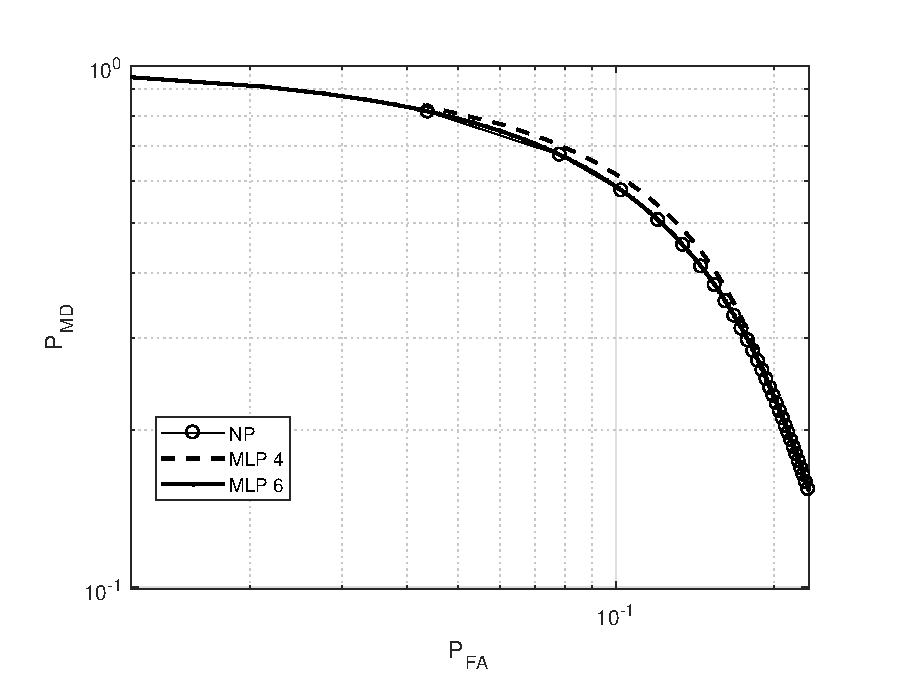
\includegraphics[width=1\columnwidth]{FA_MD_LOS.eps}
     \caption{\ac{md} probability vs. the \ac{fa} probability of the \ac{mlp} and of the optimal classificator. The number that follows \ac{mlp} indicates the number of neurons in the hidden layer.}
     \label{fig:NP_comp}
 \end{figure}


\subsection{Non-LOS Case}
We here consider a network with $N_{\rm BS}=5$ \acp{bs}, each one gathering attenuation values of \ac{ue} transmitted signal and collect them in the attenuation vector $\bm{a}$. Each \ac{bs} is characterized by different attenuation and shadowing map. Figure \ref{fig:trueMap} shows a realization of the path loss and shadowing map for a \ac{bs} located at the center of area $\mathcal{A}$. We further assume that within $\mathcal{A}$ are present two orthogonal \ac{los} paths traversing the center of $\mathcal{A}$. We define the legitimate area as the one contoured by the red line.


\begin{figure}[t]
    \centering
    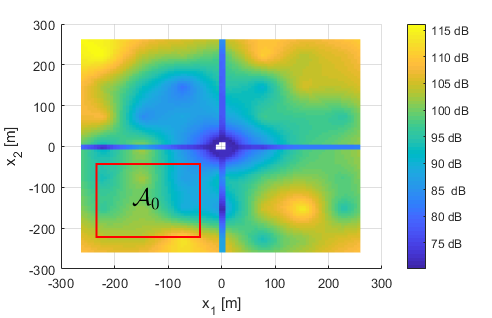
\includegraphics[width=1\columnwidth]{surfColorato.png}
    \caption{Example of a realization of the attenuation map in the non-\ac{los} scenario considering only the shadowing effects.}
    \label{fig:trueMap}
\end{figure}

Given many realization of the maps for all the $N_{\rm BS}$ we can compute the average \ac{fa} and \ac{md} probabilities of the authentication system.

Fig. \ref{fig:n_train} shows the average \ac{md} vs. \ac{fa} probabilities of the authentication system trained with $n_{train} = 10, 100, 1000$ and $10000$ points. We see that as the number of training points increases the average performance of the system increase.

\begin{figure}[t]
    \centering
    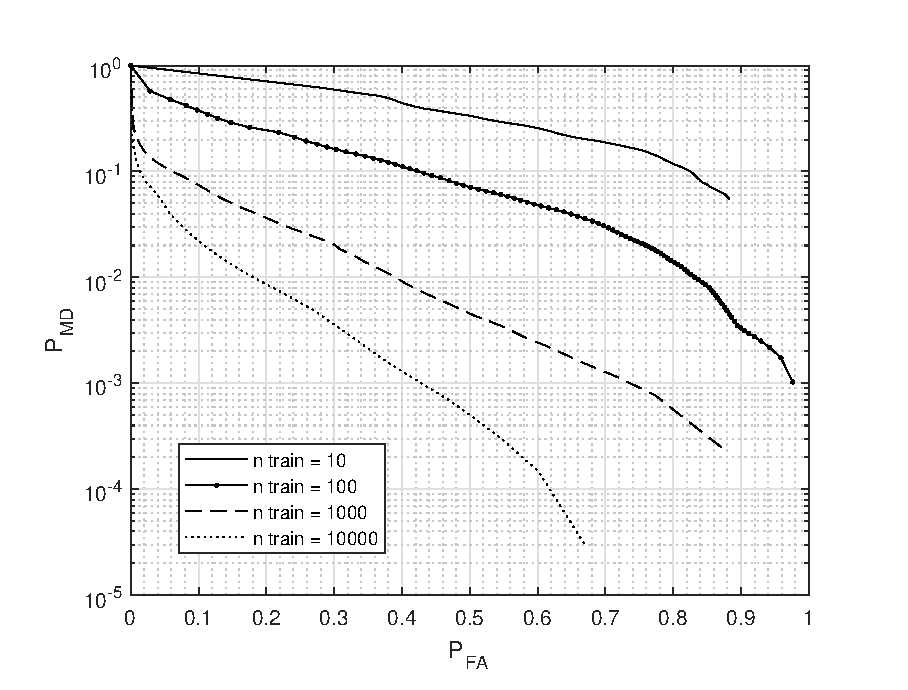
\includegraphics[width=1\columnwidth]{mean_maps.eps}
    \caption{Average \ac{md} vs. average \ac{fa} probabilities of the authentication system trained with different number of attenuation vectors.}
    \label{fig:n_train}
\end{figure}

\subsection{BSs Positioning}
We here consider the optimization Algorithm shown in Algorithm 1. We consider a \ac{pso} with $P=6$ particles, each composed by a set of $N_{\rm BS}=5$ \acp{bs} initialized with random positions. We initialize the parameters of the \ac{pso}, i.e., the inertia coefficient and the acceleration constants with the typical values $w=0.7298$, $c_1=c_2=1.4961$ \cite{Kennedy-11}. We consider different realizations of the shadowing map and obtained results are averaged over this realization. We consider a training set composed by $10^4$ points and a testing set of $10^3$ points.

Fig. \ref{fig:CE} shows the average \ac{ce} obtained by the global best particle vs. the considered \ac{pso} iteration. We see that as particles move the average \ac{ce} values decreases.

Fig. \ref{fig:CEvsAUC} shows the average \ac{auc} value vs. the number of iterations. In particular Fig. \ref{fig:CEvsAUC} compares the average \ac{auc} value obtained by training different \acp{nn} for each particle and optimizing the \ac{auc} with the \ac{auc} that would be obtained if testing the \ac{nn} that guarantees minimum \ac{ce}. We see that the \ac{auc} of the minimum \ac{ce} network is close to the one obtained by the minimum \ac{auc} network. This confirms our intuition that the \ac{ce} can be used as a proxy for the \ac{auc} and that \ac{pso} can be implemented without testing each \ac{nn} that would be needed for the different particles and their positions.

\begin{figure}[t]
    \centering
    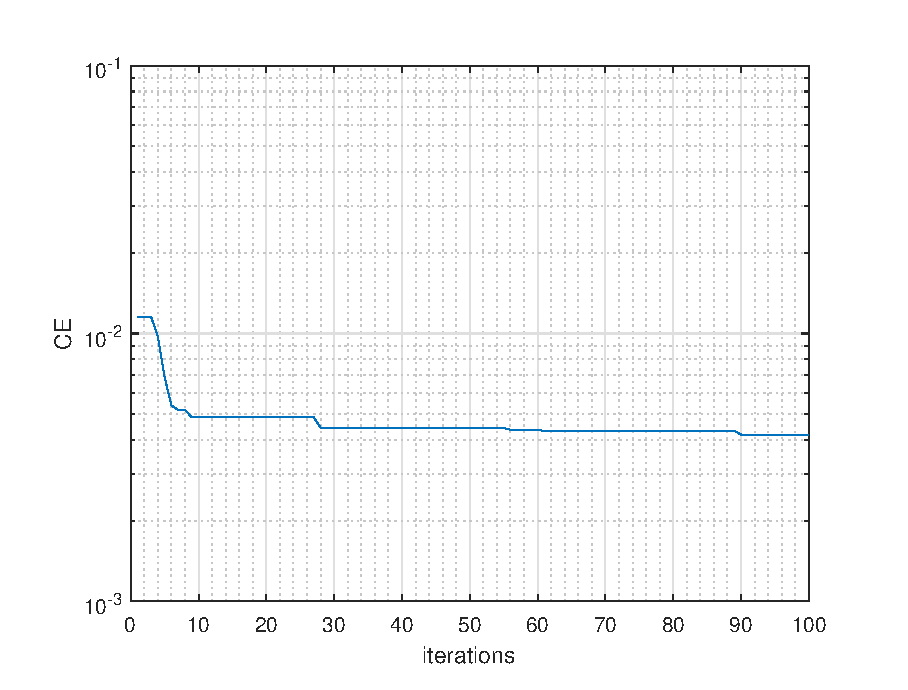
\includegraphics[width=1\columnwidth]{CE_3.eps}
    \caption{Mean \ac{ce} vs. number of \ac{pso} iterations.}
    \label{fig:CE}
\end{figure}

\begin{figure}[t]
    \centering
    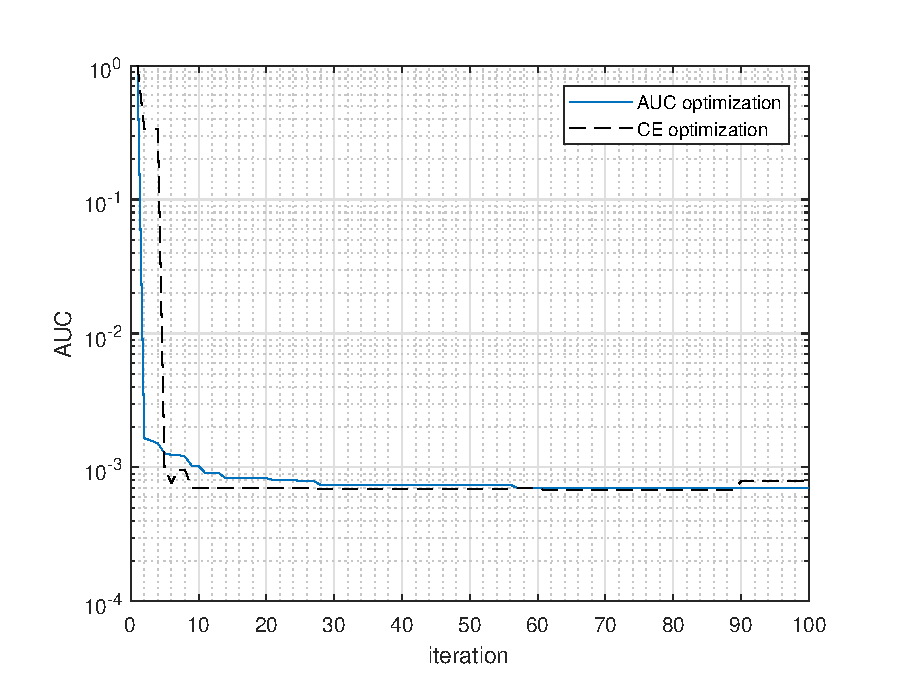
\includegraphics[width=1\columnwidth]{CE_vsAUC.eps}
    \caption{Mean \ac{auc} vs. number of \ac{pso} iterations. Comparison between the \ac{auc} obtained with testing and \ac{auc} obtained if testing the position that guarantees minimum \ac{ce}.}
    \label{fig:CEvsAUC}
\end{figure}


\renewcommand*{\bibfont}{\footnotesize}

\printbibliography
\balance
\end{document}
